\documentclass[11pt,letterpaper]{article}
\usepackage[utf8]{inputenc}
\usepackage[T1]{fontenc}
\usepackage{lmodern}
\usepackage[margin=1in]{geometry}
\usepackage{amsmath,amssymb,amsfonts,amsthm}
\usepackage{booktabs}
\usepackage{microtype}
\usepackage{enumitem}
\usepackage{fancyhdr}
\usepackage{titlesec}
\usepackage{xcolor}
\usepackage{tikz}
\usepackage{pgfplots}
\usepackage{mdframed}
\usepackage[hidelinks,colorlinks=true,linkcolor=SlateBlue,citecolor=SlateBlue,urlcolor=Terracotta]{hyperref}

\pgfplotsset{compat=1.18}
\usetikzlibrary{arrows.meta,positioning,calc,patterns,decorations.pathreplacing}

\definecolor{SlateBlue}{HTML}{1E293B}
\definecolor{Terracotta}{HTML}{C2410C}
\definecolor{ForestGreen}{HTML}{15803D}
\definecolor{LightSlate}{HTML}{F8FAFC}
\definecolor{BorderGray}{HTML}{CBD5E1}
\definecolor{LightTerracotta}{HTML}{FFF7ED}
\definecolor{CourseBlue}{HTML}{0072B2}
\definecolor{CourseOrange}{HTML}{D55E00}
\definecolor{CourseTeal}{HTML}{009E73}
\definecolor{CoursePurple}{HTML}{CC79A7}
\definecolor{CourseAmber}{HTML}{E69F00}

\titleformat{\section}{\normalfont\Large\bfseries\color{SlateBlue}}{\thesection}{1em}{}[\titlerule]
\titleformat{\subsection}{\normalfont\large\bfseries\color{SlateBlue}}{\thesubsection}{1em}{}
\titleformat{\subsubsection}{\normalfont\normalsize\bfseries\color{Terracotta}}{\thesubsubsection}{1em}{}

\pagestyle{fancy}
\fancyhf{}
\renewcommand{\headrulewidth}{0.4pt}
\renewcommand{\footrulewidth}{0.4pt}
\fancyhead[L]{\small\scshape\color{SlateBlue}\leftmark}
\fancyhead[R]{\small\color{SlateBlue}Principles of Economics}
\fancyfoot[C]{\thepage}

\newmdenv[
  linecolor=Terracotta,
  linewidth=1.5pt,
  backgroundcolor=LightTerracotta,
  innertopmargin=10pt,
  innerbottommargin=10pt,
  innerrightmargin=12pt,
  innerleftmargin=12pt,
  roundcorner=4pt,
  skipabove=12pt,
  skipbelow=12pt
]{coreprinciple}

\newmdenv[
  linecolor=SlateBlue,
  linewidth=1.5pt,
  backgroundcolor=LightSlate,
  innertopmargin=10pt,
  innerbottommargin=10pt,
  innerrightmargin=12pt,
  innerleftmargin=12pt,
  roundcorner=4pt,
  skipabove=12pt,
  skipbelow=12pt
]{casestudy}

\newenvironment{examplecase}[1]{%
  \begin{casestudy}
  \boxheader{SlateBlue}{#1}
  \vspace{0.4em}
}{%
  \end{casestudy}
}

\newmdenv[
  linecolor=BorderGray,
  linewidth=1pt,
  backgroundcolor=white,
  innertopmargin=10pt,
  innerbottommargin=10pt,
  innerrightmargin=12pt,
  innerleftmargin=12pt,
  roundcorner=4pt,
  skipabove=12pt,
  skipbelow=12pt
]{takeaways}

\newcommand{\boxheader}[2]{{\noindent\bfseries\color{#1}\Large #2}\vspace{0.4em}\par}

% ==============================================================================
% TikZ & PGFPlots Global Configuration and Economics Styling
% ==============================================================================

\usepackage{tikz}
\usepackage{pgfplots}
\pgfplotsset{compat=1.18}

% TikZ Libraries
\usetikzlibrary{
    arrows.meta,
    positioning,
    calc,
    shapes.geometric,
    patterns,
    decorations.pathreplacing,
    intersections
}

% Common Economics TikZ Styles
\tikzset{
    % Axes and Structural Lines
    econ axis/.style={->, >=Stealth, thick, color=SlateBlue!90!black},
    econ grid/.style={thin, dashed, color=gray!30},
    econ guide/.style={dashed, color=gray!60, thin},
    % Curves and Functions
    demand curve/.style={very thick, color=SlateBlue},
    supply curve/.style={very thick, color=Terracotta},
    mb curve/.style={very thick, color=SlateBlue},
    mc curve/.style={very thick, color=Terracotta},
    % Points and Highlights
    econ point/.style={circle, fill=SlateBlue!90!black, inner sep=1.8pt},
    econ highlight/.style={fill=Terracotta!20, opacity=0.5},
    % Annotations
    econ label/.style={font=\small\sffamily, align=center},
    econ annotation/.style={font=\footnotesize\itshape, color=SlateBlue!80!black}
}

% PGFPlots Standard Economics Style
\pgfplotsset{
    econ diagram/.style={
        axis lines=left,
        xlabel style={at={(ticklabel* cs:1)}, anchor=north west, font=\small\bfseries},
        ylabel style={at={(ticklabel* cs:1)}, anchor=south east, font=\small\bfseries},
        label style={font=\small},
        tick label style={font=\small},
        grid=none,
        enlargelimits=false,
        axis line style={->, >=Stealth, thick, color=SlateBlue!90!black}
    }
}

\usepackage{tcolorbox}

\begin{document}

\title{\Huge\bfseries\color{SlateBlue} Chapter 9: Monopolistic Competition, Oligopoly, and Game Theory}
\author{\large Principles of Microeconomics Curriculum}
\date{2026}
\maketitle

\thispagestyle{plain}

\begin{abstract}
This chapter provides a rigorous, algebra-first treatment of imperfect competition—monopolistic competition, oligopoly, and strategic game theory—benchmarked to the Principles of Microeconomics curriculum (Eric Chiang framework).
\end{abstract}

\tableofcontents
\vspace{1.5em}
\hrule
\vspace{1.5em}

\begin{examplecase}{Bring It Home: Why Do Coffee Shops Proliferate While Wireless Carriers Dominate?}
Walk through almost any college neighborhood and you can choose among half a dozen cafés—one roasting single-origin pour-overs, another offering matcha lattes and study tables, and a third specializing in quick espresso—yet your phone connects to one of only a few major national wireless carriers. Why can a new café open on a corner storefront while launching a new nationwide cellular network is nearly impossible? And why do competing streaming platforms or airlines constantly monitor and react to one another's price cuts? This chapter explains how \textbf{product differentiation}, \textbf{barriers to entry}, and \textbf{strategic interdependence} shape prices, profits, and consumer welfare in markets that fall between perfect competition and pure monopoly.
\end{examplecase}

% -----------------------------------------------------------------------------
% Section 9.1: Monopolistic Competition and Excess Capacity
% -----------------------------------------------------------------------------
\section{Monopolistic Competition and Excess Capacity}

\subsection*{Conceptual Introduction}
Most everyday consumer markets—coffee shops, hair salons, casual restaurants, fitness studios, and clothing boutiques—do not fit neatly into either perfect competition or pure monopoly. Instead, they operate under \textbf{monopolistic competition}, a hybrid market structure combining three defining traits: (1) many competing sellers, (2) \textbf{differentiated products} (each seller offers a distinct flavor, location, brand aesthetic, or customer experience, often reinforced through \textbf{non-price competition} such as branding and advertising), and (3) \textbf{free entry and exit} in the long run.

Because its product is distinct from rivals, each monopolistically competitive firm enjoys a small degree of brand loyalty and faces a \textbf{downward-sloping demand curve}. Just like a monopolist, the firm maximizes short-run profit by producing where Marginal Revenue equals Marginal Cost ($MR = MC$) and pricing on its demand curve ($P > MC$). However, because there are zero barriers to entry, positive short-run economic profits attract new competitors into the neighborhood—drawing away customers and shifting each incumbent firm's demand curve inward until economic profits are driven to zero. Conversely, short-run economic losses cause some firms to exit, shifting remaining firms' demand outward until losses disappear.

In long-run equilibrium, the firm's downward-sloping demand curve becomes tangent to its Average Total Cost ($ATC$) curve, enforcing zero economic profit ($P = ATC$). Yet unlike perfect competition, this tangency occurs strictly to the left of minimum $ATC$, creating two permanent structural features: a \textbf{markup over marginal cost} ($P > MC$, implying allocative inefficiency) and \textbf{excess capacity} ($q_{\text{LR}} < q_{\text{eff}}$, implying productive inefficiency). Rather than pure waste, however, this tradeoff reflects the price society pays for product variety and convenience.

\begin{tcolorbox}[colback=LightTerracotta,colframe=CourseOrange,title=\textbf{Clear It Up: Zero Economic Profit and Excess Capacity}]
Two common misconceptions arise in monopolistic competition:
\begin{enumerate}
    \item \textbf{Zero economic profit does \emph{not} mean zero accounting profit.} At $P_{\text{LR}} = ATC$, the owner earns a \emph{normal profit}—covering all explicit bills (rent, wages, supplies) plus the full opportunity cost of the owner's time and invested capital.
    \item \textbf{Excess capacity is not necessarily harmful.} Producing below minimum $ATC$ raises average cost slightly, yet consumers willingly pay a small markup to enjoy diverse neighborhood options rather than one standardized product.
\end{enumerate}
\end{tcolorbox}

\subsection*{Visual Representation}
Figure~\ref{fig:monopolistic_competition} illustrates the long-run zero-profit equilibrium of a monopolistically competitive firm, highlighting the tangency between demand and $ATC$, the $MR = MC$ profit-maximizing output, and the resulting excess capacity gap.

\begin{figure}[htbp]
\centering
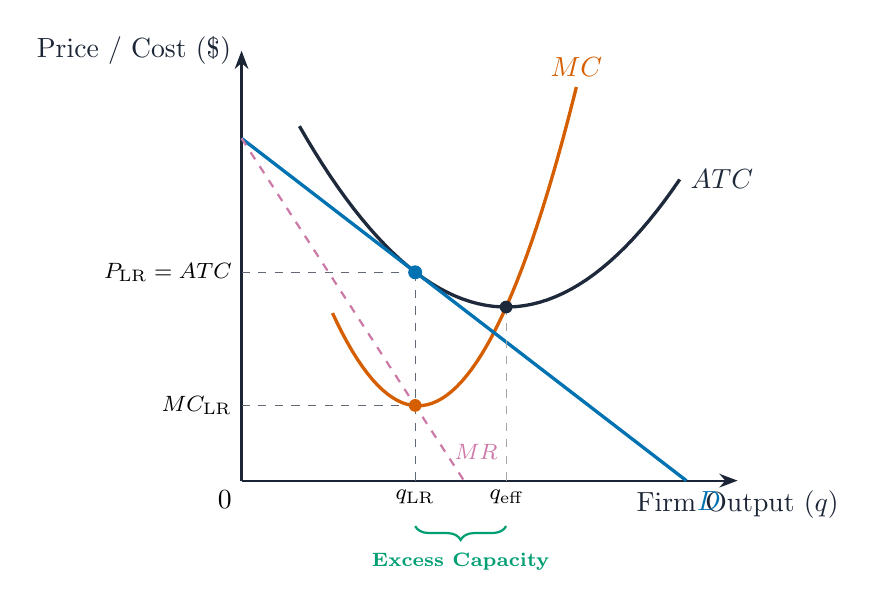
\begin{tikzpicture}[scale=1.05]
    % Axes
    \draw[->, >=Stealth, thick, color=SlateBlue!90!black] (0,0) -- (6.0,0) node[below] {Firm Output ($q$)};
    \draw[->, >=Stealth, thick, color=SlateBlue!90!black] (0,0) -- (0,5.2) node[left] {Price / Cost (\$)};
    \node[below left] at (0,0) {$0$};

    % ATC curve: min at x=3.2, y=2.1 -> y = 2.1 + 0.35*(x-3.2)^2
    \draw[very thick, color=SlateBlue, domain=0.7:5.3, samples=50] plot (\x, {2.1 + 0.35*(\x-3.2)*(\x-3.2)}) node[right] {$ATC$};

    % MC curve: d(x*ATC)/dx = 2.1 + 0.35*(x-3.2)^2 + 0.7*x*(x-3.2); MC(4.05)=4.76 < 5.2
    \draw[very thick, color=CourseOrange, domain=1.1:4.05, samples=50] plot (\x, {2.1 + 0.35*(\x-3.2)*(\x-3.2) + 0.7*\x*(\x-3.2)}) node[above] {$MC$};

    % Tangency at q_LR = 2.1: ATC(2.1) = 2.5235; slope of ATC at 2.1 = -0.77
    % Demand line: y = 4.1405 - 0.77x (x-int at 5.38)
    \draw[very thick, color=CourseBlue] (0,4.14) -- (5.38,0) node[below right] {$D$};
    % MR line: y = 4.1405 - 1.54x (x-int at 2.69)
    \draw[thick, dashed, color=CoursePurple] (0,4.14) -- (2.69,0);
    \node[right, font=\footnotesize, color=CoursePurple] at (2.46,0.35) {$MR$};

    % Equilibrium projections at q_LR = 2.1, P_LR = 2.52, MC_LR = 0.91
    \draw[dashed, color=SlateBlue!70] (0,2.52) node[left, color=black, font=\footnotesize] {$P_{\text{LR}} = ATC$} -- (2.1,2.52);
    \draw[dashed, color=SlateBlue!70] (0,0.91) node[left, color=black, font=\footnotesize] {$MC_{\text{LR}}$} -- (2.1,0.91);
    \draw[dashed, color=SlateBlue!70] (2.1,0) node[below, color=black, font=\footnotesize] {$q_{\text{LR}}$} -- (2.1,2.52);
    \filldraw[CourseBlue] (2.1,2.52) circle (2.2pt);
    \filldraw[CourseOrange] (2.1,0.91) circle (2.0pt);

    % Efficient scale projection at q_eff = 3.2
    \draw[dashed, color=gray!70] (3.2,0) node[below, color=black, font=\footnotesize] {$q_{\text{eff}}$} -- (3.2,2.1);
    \filldraw[SlateBlue] (3.2,2.1) circle (2.0pt);

    % Excess capacity under-brace cleanly below x-axis (zero curve overlap)
    \draw[decorate, decoration={brace, amplitude=5pt, mirror}, thick, color=CourseTeal] (2.1,-0.55) -- (3.2,-0.55)
        node[midway, below=6pt, font=\scriptsize\bfseries, color=CourseTeal] {Excess Capacity};
\end{tikzpicture}
\caption{Long-Run Equilibrium under Monopolistic Competition. Free entry shifts demand until it is tangent to $ATC$ at $q_{\text{LR}}$ (where $MR = MC$), yielding zero economic profit ($P_{\text{LR}} = ATC$). Because $q_{\text{LR}} < q_{\text{eff}}$, the firm operates with excess capacity and charges a markup above $MC_{\text{LR}}$.}
\label{fig:monopolistic_competition}
\end{figure}

\subsection*{Real-World Application: Neighborhood Coffee Shops and Retail Differentiation}
Walk down any busy commercial avenue and you will see independent cafés every two blocks—one roasting single-origin pour-overs, another offering oat-milk matcha and study booths, and a third specializing in quick drive-thru espresso. None earns monopoly-level economic profits for long because new cafés open whenever neighborhood rents permit, yet each operates below its physical kitchen capacity during mid-afternoon lulls so consumers can enjoy variety and convenience.

\subsection*{Mathematical Foundation (Algebra Level)}
In long-run monopolistic competition, two simultaneous conditions hold at output $q_{\text{LR}}$:
\begin{equation}
MR(q_{\text{LR}}) = MC(q_{\text{LR}}) \quad \text{(Profit Maximization)}, \qquad P(q_{\text{LR}}) = ATC(q_{\text{LR}}) \quad \text{(Zero Economic Profit)}
\end{equation}

\begin{tcolorbox}[colback=LightSlate,colframe=CourseTeal,title=\textbf{Work It Out: Long-Run Equilibrium for a Boutique Fitness Studio}]
\noindent\textbf{Problem:}
Assume a boutique fitness studio in a monopolistically competitive neighborhood faces a linear long-run inverse demand curve $P = 50 - 2q$ (where $P$ is class price in dollars and $q$ is daily clients) and corresponding Marginal Revenue $MR = 50 - 4q$. Suppose the studio has fixed daily overhead of $\$200$ and constant Marginal Cost $MC = \$10$ per client, giving Average Total Cost $ATC = \frac{200}{q} + 10$ (which declines over the studio's operating range).
\begin{enumerate}
    \item Find the studio's profit-maximizing client volume $q_{\text{LR}}$ and class price $P_{\text{LR}}$.
    \item Verify that the studio earns zero economic profit in the long run.
    \item Calculate the firm's markup over marginal cost ($P_{\text{LR}} - MC$).
\end{enumerate}

\noindent\textbf{Step-by-Step Solution:}
\begin{enumerate}
    \item \textbf{Set $MR = MC$ to Solve for $q_{\text{LR}}$ and $P_{\text{LR}}$:}
    \[
    50 - 4q_{\text{LR}} = 10 \implies 4q_{\text{LR}} = 40 \implies q_{\text{LR}} = \mathbf{10\text{ clients per day}}
    \]
    Substitute $q_{\text{LR}} = 10$ into the inverse demand curve:
    \[
    P_{\text{LR}} = 50 - 2(10) = \mathbf{\$30\text{ per class}}
    \]

    \item \textbf{Check Long-Run Economic Profit ($\pi$):}
    Compute $ATC$ at $q_{\text{LR}} = 10$:
    \[
    ATC(10) = \frac{200}{10} + 10 = 20 + 10 = \$30\text{ per class}
    \]
    Since $P_{\text{LR}}\ (\$30) = ATC\ (\$30)$, economic profit is:
    \[
    \pi = (\$30 - \$30) \times 10 = \mathbf{\$0}
    \]

    \item \textbf{Compute the Markup over Marginal Cost:}
    \[
    \text{Markup} = P_{\text{LR}} - MC = \$30 - \$10 = \mathbf{\$20\text{ per class}}
    \]
\end{enumerate}
\textbf{Conclusion:} The studio breaks even in economic terms ($\pi = \$0$) while maintaining a $\$20$ markup above marginal cost due to product differentiation.
\end{tcolorbox}

\begin{tcolorbox}[colback=LightSlate,colframe=CourseBlue,title=\textbf{Optional Advanced Section: Proving Tangency and Excess Capacity}]
\small
\emph{Note for Economics Majors and Quantitative Students:}
Write economic profit as $\pi(q) = q\bigl[P(q) - ATC(q)\bigr]$. In long-run equilibrium at $q_{\text{LR}} > 0$, both zero profit ($\pi(q_{\text{LR}}) = 0 \implies P(q_{\text{LR}}) = ATC(q_{\text{LR}})$) and profit maximization ($\pi'(q_{\text{LR}}) = 0$) must hold. Applying the product rule:
\[
\pi'(q_{\text{LR}}) = \underbrace{\bigl[P(q_{\text{LR}}) - ATC(q_{\text{LR}})\bigr]}_{=\,0} + q_{\text{LR}}\bigl[P'(q_{\text{LR}}) - ATC'(q_{\text{LR}})\bigr] = 0
\]
Because $q_{\text{LR}} > 0$, this forces $P'(q_{\text{LR}}) = ATC'(q_{\text{LR}})$, proving that the demand curve is \textbf{tangent} to $ATC$ at $q_{\text{LR}}$. Moreover, since downward-sloping demand implies $P'(q_{\text{LR}}) < 0$, it follows that $ATC'(q_{\text{LR}}) < 0$: the firm must operate strictly to the left of minimum $ATC$, mathematically guaranteeing excess capacity. (In the fitness studio problem above, $P'(10) = -2$ and $ATC'(10) = -200/10^2 = -2$, confirming exact tangency.)
\end{tcolorbox}

% -----------------------------------------------------------------------------
% Section 9.2: Oligopoly, Cartels, and Strategic Interdependence
% -----------------------------------------------------------------------------
\section{Oligopoly, Cartels, and Strategic Interdependence}

\subsection*{Conceptual Introduction}
When an industry is dominated by just a handful of large firms—such as commercial aircraft manufacturing (Boeing and Airbus), wireless telecom carriers, or major airlines—the market is an \textbf{oligopoly}. Unlike monopolistically competitive markets with easy entry, oligopolies are protected by \textbf{significant barriers to entry}, including large economies of scale, control of scarce spectrum licenses, patents, or network effects. Because only a few rivals share the market, oligopolists are acutely aware of one another: every pricing decision, advertising campaign, or product launch by one firm directly affects its rivals' sales and triggers counter-moves. Economists call this mutual awareness \textbf{strategic interdependence}.

Because oligopolists control the bulk of market supply, they face a powerful temptation to collude—forming a formal or informal \textbf{cartel} to restrict industry output and hold prices up near the monopoly level so they can split monopoly profits. However, cartels suffer from an inherent internal instability. Once a cartel sets a high price above marginal cost ($P > MC$), each individual member realizes it can secretly undercut the agreed price slightly, steal its rivals' customers, and boost its own profit—until all members cheat and prices collapse back toward competitive levels.

Economists measure industry concentration using two standard tools: the \textbf{Four-Firm Concentration Ratio ($CR_4$)}, which sums the market shares of the four largest firms, and the \textbf{Herfindahl-Hirschman Index ($HHI$)}, which sums the squared market shares of all firms in the market ($HHI = \sum_{i=1}^N s_i^2$). Antitrust regulators at the Department of Justice and Federal Trade Commission scrutinize mergers that sharply increase the $HHI$.

\subsection*{Visual Representation}
Figure~\ref{fig:oligopoly_spectrum} contrasts market outcomes along a quantity-price continuum under linear market demand and constant marginal cost, showing how a non-cooperative oligopoly settles strictly between the collusive cartel benchmark ($Q_{\text{cartel}}, P_{\text{cartel}}$) and the competitive benchmark ($Q_C, P_C$).

\begin{figure}[htbp]
\centering
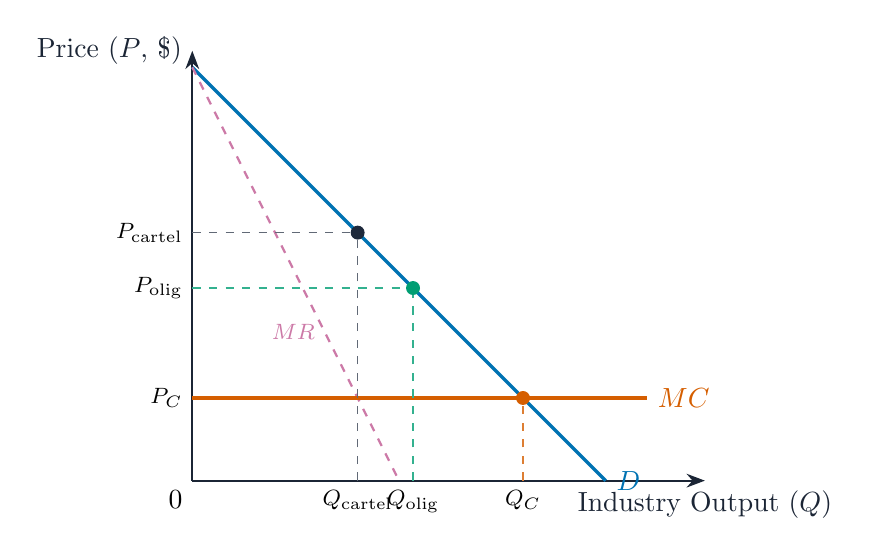
\begin{tikzpicture}[scale=1.05]
    % Axes
    \draw[->, >=Stealth, thick, color=SlateBlue!90!black] (0,0) -- (6.2,0) node[below] {Industry Output ($Q$)};
    \draw[->, >=Stealth, thick, color=SlateBlue!90!black] (0,0) -- (0,5.2) node[left] {Price ($P$, \$)};
    \node[below left] at (0,0) {$0$};

    % Demand: P = 100 - 2Q -> (0,5) to (5,0)
    \draw[very thick, color=CourseBlue] (0,5.0) -- (5.0,0) node[right] {$D$};
    % MR: P = 100 - 4Q -> (0,5) to (2.5,0)
    \draw[thick, dashed, color=CoursePurple] (0,5.0) -- (2.5,0);
    \node[left, font=\footnotesize, color=CoursePurple] at (1.60,1.80) {$MR$};
    % Constant MC = $20 -> y = 1.0
    \draw[very thick, color=CourseOrange] (0,1.0) -- (5.5,1.0) node[right] {$MC$};
    \node[left, font=\footnotesize] at (0,1.0) {$P_C$};

    % Monopoly / Cartel Outcome: Q_M = 20 (x=2.0), P_M = $60 (y=3.0)
    \draw[dashed, color=SlateBlue!70] (0,3.0) node[left, color=black, font=\footnotesize] {$P_{\text{cartel}}$} -- (2.0,3.0);
    \draw[dashed, color=SlateBlue!70] (2.0,0) node[below, color=black, font=\footnotesize] {$Q_{\text{cartel}}$} -- (2.0,3.0);
    \filldraw[SlateBlue] (2.0,3.0) circle (2.2pt);

    % Duopoly / Oligopoly Outcome: Q_olig = 26.67 (x=2.67), P_olig = $46.67 (y=2.33)
    \draw[dashed, color=CourseTeal!80] (0,2.33) node[left, color=black, font=\footnotesize] {$P_{\text{olig}}$} -- (2.67,2.33);
    \draw[dashed, color=CourseTeal!80] (2.67,0) node[below, color=black, font=\footnotesize] {$Q_{\text{olig}}$} -- (2.67,2.33);
    \filldraw[CourseTeal] (2.67,2.33) circle (2.2pt);

    % Competitive Outcome: Q_C = 40 (x=4.0), P_C = $20 (y=1.0)
    \draw[dashed, color=CourseOrange!80] (4.0,0) node[below, color=black, font=\footnotesize] {$Q_C$} -- (4.0,1.0);
    \filldraw[CourseOrange] (4.0,1.0) circle (2.2pt);
\end{tikzpicture}
\caption{The Oligopoly Output-Price Spectrum. When oligopolists fail to sustain a cartel, non-cooperative competition expands industry output beyond $Q_{\text{cartel}}$ and lowers price below $P_{\text{cartel}}$, moving the market closer to the competitive outcome $(Q_C, P_C)$.}
\label{fig:oligopoly_spectrum}
\end{figure}

\subsection*{Real-World Application: OPEC Production Quotas and Cheating Incentives}
The Organization of the Petroleum Exporting Countries (OPEC) acts as an international oil cartel, agreeing on production quotas to keep global crude oil prices elevated. As an illustrative example, if OPEC restricts output and pushes crude oil to $\$90$ per barrel while a member country's marginal extraction cost is only $\$20$ per barrel, that member faces an immediate temptation to quietly pump above its assigned quota—earning an extra $\$70$ per barrel—until rival members detect the cheating and quotas break down.

\subsection*{Mathematical Foundation (Algebra Level)}
The Herfindahl-Hirschman Index ($HHI$) squares each firm's percentage market share $s_i$ (expressed as a number from $0$ to $100$):
\begin{equation}
HHI = s_1^2 + s_2^2 + \dots + s_N^2
\end{equation}
A pure monopoly ($s_1 = 100$) has the maximum $HHI = 100^2 = 10{,}000$, whereas an industry split among many tiny firms approaches $HHI \approx 0$.

\begin{tcolorbox}[colback=LightSlate,colframe=CourseTeal,title=\textbf{Work It Out: Measuring Concentration and Evaluating a Horizontal Merger}]
\noindent\textbf{Problem:}
Suppose a regional wireless internet market is served by four providers with market shares of $40\%$, $30\%$, $20\%$, and $10\%$.
\begin{enumerate}
    \item Compute the Four-Firm Concentration Ratio ($CR_4$) and the baseline $HHI$.
    \item Compute the new post-merger $HHI$ and the change in $HHI$ ($\Delta HHI$) if the two smallest providers ($20\%$ and $10\%$) merge into a single $30\%$ firm (assuming customer shares initially combine without defection).
\end{enumerate}

\noindent\textbf{Step-by-Step Solution:}
\begin{enumerate}
    \item \textbf{Calculate Baseline $CR_4$ and $HHI$:}
    \[
    CR_4 = 40\% + 30\% + 20\% + 10\% = \mathbf{100\%}
    \]
    \[
    HHI_{\text{pre}} = 40^2 + 30^2 + 20^2 + 10^2 = 1{,}600 + 900 + 400 + 100 = \mathbf{3{,}000}
    \]

    \item \textbf{Calculate Post-Merger $HHI$ (Shares: $40\%$, $30\%$, $30\%$) and $\Delta HHI$:}
    \[
    HHI_{\text{post}} = 40^2 + 30^2 + 30^2 = 1{,}600 + 900 + 900 = \mathbf{3{,}400}
    \]
    \[
    \Delta HHI = HHI_{\text{post}} - HHI_{\text{pre}} = 3{,}400 - 3{,}000 = \mathbf{+400\text{ points}}
    \]
    \emph{Algebraic check:} When two firms with shares $s_A$ and $s_B$ merge, $(s_A + s_B)^2 - (s_A^2 + s_B^2) = 2 s_A s_B = 2(20)(10) = 400$.
\end{enumerate}
\textbf{Conclusion:} Notice that $CR_4$ stays unchanged at $100\%$, yet the $HHI$ rises by $400$ points (from $3{,}000$ to $3{,}400$), highlighting why antitrust regulators rely on $HHI$ to flag highly concentrated oligopoly mergers for review.
\end{tcolorbox}

% -----------------------------------------------------------------------------
% Section 9.3: Game Theory, Dominant Strategies, and Nash Equilibrium
% -----------------------------------------------------------------------------
\section{Game Theory, Dominant Strategies, and Nash Equilibrium}

\subsection*{Conceptual Introduction}
Because oligopolists cannot make decisions in a vacuum, economists analyze their behavior using \textbf{game theory}—the mathematical study of strategic decision-making when each player's payoff depends on the actions of other players. Every strategic game consists of three building blocks: (1) the \textbf{players}, (2) the \textbf{strategies} available to each player, and (3) the \textbf{payoffs} resulting from every combination of choices.

To predict how rational rivals will behave without binding contracts, economists look for two key concepts:
\begin{itemize}
    \item \textbf{Dominant Strategy:} A strategy that yields a strictly higher payoff for a player \emph{no matter what strategy the rival chooses}. If a player has a dominant strategy, they will always play it.
    \item \textbf{Nash Equilibrium:} An outcome in which \textbf{every player is choosing their best response given what the other players are doing}. At a Nash equilibrium, no player can improve their own payoff by unilaterally changing their strategy.
\end{itemize}

The most famous game in economics is the \textbf{Prisoner's Dilemma}. In this game, both firms could earn higher joint profits by cooperating (e.g., keeping prices high or limiting advertising), yet each firm's individual dominant strategy is to defect (slash prices or flood the market with ads). As a result, rational self-interest locks both firms into a non-cooperative Nash equilibrium where both earn lower profits!

\subsection*{Visual Representation}
Figure~\ref{fig:prisoners_dilemma} presents a $2 \times 2$ payoff matrix for two competing streaming platforms deciding simultaneously between keeping subscription prices high ($\$18$) or discounting to capture subscribers ($\$12$).

\begin{tcolorbox}[colback=LightTerracotta,colframe=CourseOrange,title=\textbf{Clear It Up: Why Prisoners' Dilemmas Are Good News for Consumers}]
In a business pricing game, failure to cooperate traps rival firms in a low-price Nash equilibrium—which hurts the firms' combined profits, yet \textbf{benefits consumers} through lower prices and higher consumer surplus! Antitrust laws exist specifically to prevent oligopolists from escaping their Prisoner's Dilemma through illegal price-fixing agreements.
\end{tcolorbox}

\begin{figure}[htbp]
\centering
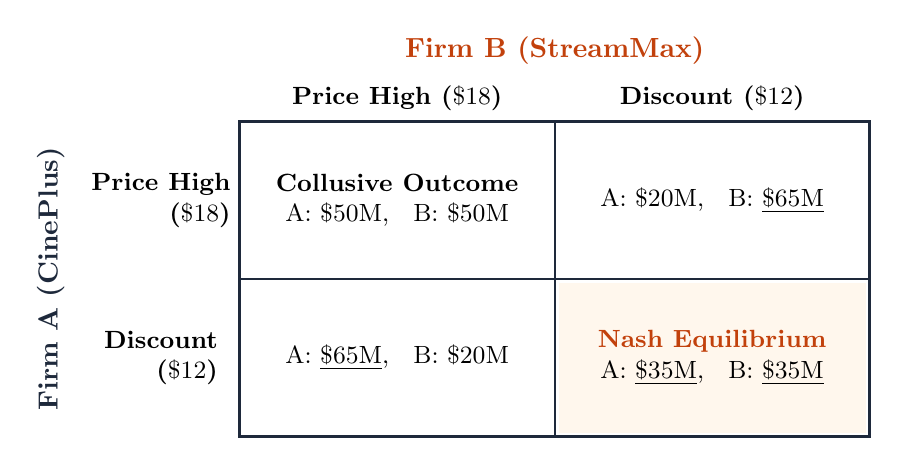
\begin{tikzpicture}[scale=1.0]
    % Grid coordinates: 2x2 matrix from (0,0) to (8,4)
    \draw[very thick, SlateBlue] (0,0) rectangle (8,4);
    \draw[thick, SlateBlue] (4,0) -- (4,4);
    \draw[thick, SlateBlue] (0,2) -- (8,2);

    % Column Headers (Firm B)
    \node[font=\bfseries\color{Terracotta}] at (4,4.9) {Firm B (StreamMax)};
    \node[font=\small\bfseries] at (2,4.3) {Price High ($\$18$)};
    \node[font=\small\bfseries] at (6,4.3) {Discount ($\$12$)};

    % Row Headers (Firm A)
    \node[font=\bfseries\color{SlateBlue}, rotate=90] at (-2.4,2) {Firm A (CinePlus)};
    \node[font=\small\bfseries, align=right] at (-1.0,3) {Price High\\($\$18$)};
    \node[font=\small\bfseries, align=right] at (-1.0,1) {Discount\\($\$12$)};

    % Cell (High, High): Top-Left (0..4, 2..4)
    \node[align=center, font=\small] at (2,3) {\textbf{Collusive Outcome}\\A: $\$50\text{M}$, \; B: $\$50\text{M}$};

    % Cell (High, Discount): Top-Right (4..8, 2..4)
    \node[align=center, font=\small] at (6,3) {A: $\$20\text{M}$, \; B: \underline{$\$65\text{M}$}};

    % Cell (Discount, High): Bottom-Left (0..4, 0..2)
    \node[align=center, font=\small] at (2,1) {A: \underline{$\$65\text{M}$}, \; B: $\$20\text{M}$};

    % Cell (Discount, Discount): Bottom-Right (4..8, 0..2) -> Nash Equilibrium
    \fill[LightTerracotta] (4.05,0.05) rectangle (7.95,1.95);
    \node[align=center, font=\small] at (6,1) {\textbf{\color{Terracotta}Nash Equilibrium}\\A: \underline{$\$35\text{M}$}, \; B: \underline{$\$35\text{M}$}};
\end{tikzpicture}
\caption{A $2 \times 2$ Pricing Prisoner's Dilemma (Annual Profits in Millions). Underlined payoffs show each firm's best response. Both firms have a dominant strategy to Discount ($\$12$), landing in the bottom-right Nash equilibrium ($\$35\text{M}, \$35\text{M}$) rather than the cooperative outcome ($\$50\text{M}, \$50\text{M}$).}
\label{fig:prisoners_dilemma}
\end{figure}

\subsection*{Real-World Application: Airline Fare Wars and Repeated Interaction}
When two airlines compete on the same nonstop route (such as San Francisco to Los Angeles), matching a competitor's fare cut within hours via automated pricing software acts as a \textbf{tit-for-tat} enforcement mechanism. Because airlines interact repeatedly day after day rather than playing a one-shot game, the credible threat of immediate retaliation helps stabilize fares without explicit collusion.

\subsection*{Mathematical Foundation (Algebra Level)}
To solve any $2 \times 2$ simultaneous game for a Nash equilibrium, evaluate each player's conditional best responses:
\begin{equation}
\text{Strategy } s_A^* \text{ is a Best Response to } s_B^* \iff \pi_A(s_A^*, s_B^*) \ge \pi_A(s_A, s_B^*) \quad \forall s_A
\end{equation}

\begin{tcolorbox}[colback=LightSlate,colframe=CourseTeal,title=\textbf{Work It Out: Solving a Simultaneous Pricing Game}]
\noindent\textbf{Problem:}
Using the simultaneous one-shot payoff matrix in Figure~\ref{fig:prisoners_dilemma}, prove mathematically why \textbf{Discount ($\$12$)} is a strictly dominant strategy for Firm A and verify that \textbf{(Discount, Discount)} is the unique Nash equilibrium.

\noindent\textbf{Step-by-Step Solution:}
\begin{enumerate}
    \item \textbf{Check Firm A's Best Response When Firm B Plays ``Price High ($\$18$)'':}
    Compare Firm A's profit in the left column:
    \[
    \pi_A(\text{Discount} \mid \text{B High}) = \$65\text{M} > \pi_A(\text{High} \mid \text{B High}) = \$50\text{M}
    \]
    Firm A earns $\$15\text{M}$ more by discounting.

    \item \textbf{Check Firm A's Best Response When Firm B Plays ``Discount ($\$12$)'':}
    Compare Firm A's profit in the right column:
    \[
    \pi_A(\text{Discount} \mid \text{B Discount}) = \$35\text{M} > \pi_A(\text{High} \mid \text{B Discount}) = \$20\text{M}
    \]
    Firm A again earns $\$15\text{M}$ more by discounting.

    \item \textbf{Confirm Dominant Strategy and Nash Equilibrium:}
    Because Discount yields a strictly higher payoff regardless of Firm B's choice, \textbf{Discount is Firm A's strictly dominant strategy}. By symmetry, \textbf{Discount is also Firm B's strictly dominant strategy}. At \textbf{(Discount, Discount)}, neither firm can raise its profit above $\$35\text{M}$ by switching unilaterally to High (which drops its profit to $\$20\text{M}$).
\end{enumerate}
\textbf{Conclusion:} \textbf{(Discount, Discount)} with payoffs $(\$35\text{M}, \$35\text{M})$ is the unique Nash equilibrium, even though both firms would earn $\$50\text{M}$ each if they could credibly cooperate.
\end{tcolorbox}

\begin{tcolorbox}[colback=LightSlate,colframe=CourseBlue,title=\textbf{Optional Advanced Section: Cournot Duopoly Best-Response Functions}]
\small
\emph{Note for Economics Majors and Quantitative Students:}
In a continuous quantity-setting Cournot duopoly facing linear market inverse demand $P = 100 - (q_1 + q_2)$ with symmetric constant marginal cost $MC = 10$, Firm 1 chooses $q_1$ to maximize $\pi_1 = [100 - q_1 - q_2]q_1 - 10q_1 = 90q_1 - q_1^2 - q_1 q_2$. Setting $\frac{\partial \pi_1}{\partial q_1} = 90 - 2q_1 - q_2 = 0$ yields Firm 1's continuous \textbf{best-response function}:
\[
q_1^*(q_2) = 45 - \frac{1}{2}q_2
\]
By symmetry, $q_2^*(q_1) = 45 - \frac{1}{2}q_1$. Solving simultaneously gives the Cournot-Nash equilibrium output $q_1^* = q_2^* = 30$ (total output $Q = 60$, price $P = \$40$, profit $\pi_i = \$900$ each), lying strictly between the cartel output ($Q_M = 45, P_M = \$55$) and competitive output ($Q_C = 90, P_C = \$10$).
\end{tcolorbox}

\begin{takeaways}
\boxheader{SlateBlue}{Bringing It Home: Key Chapter Takeaways}
\begin{itemize}
    \item \textbf{Monopolistic Competition (Neighborhood Cafés):} Free entry eliminates long-run economic profit ($P = ATC$), while product differentiation leaves firms with a markup ($P > MC$) and excess capacity ($q_{\text{LR}} < q_{\text{eff}}$)—the tradeoff for consumer variety.
    \item \textbf{Oligopoly (Wireless Carriers):} High barriers to entry keep markets concentrated (measured by $CR_4$ and $HHI$) and make firms strategically interdependent, yielding prices and quantities between cartel and competitive benchmarks.
    \item \textbf{Game Theory (Streaming \& Airlines):} Rational rivals in a one-shot Prisoner's Dilemma follow dominant strategies into lower-profit Nash equilibria that benefit consumers, whereas repeated interaction can partially stabilize competition through tit-for-tat responses.
\end{itemize}
\end{takeaways}

\end{document}
